\chapter{Analysis Results}

The results for all on-Z regions are shown in Figure~\ref{fig:on_Z_results}, and those for all edge regions are shown in Figure~\ref{fig:edge_results}. A summary of all results are shown in Figure~\ref{fig:all_results}. As we see from these plots, data was consistent with expected backgrounds from only Standard Model processes in all regions.

Ah well, guess we didn't find anything after all. The search goes on!

\begin{figure}[htbp]
    \centering
    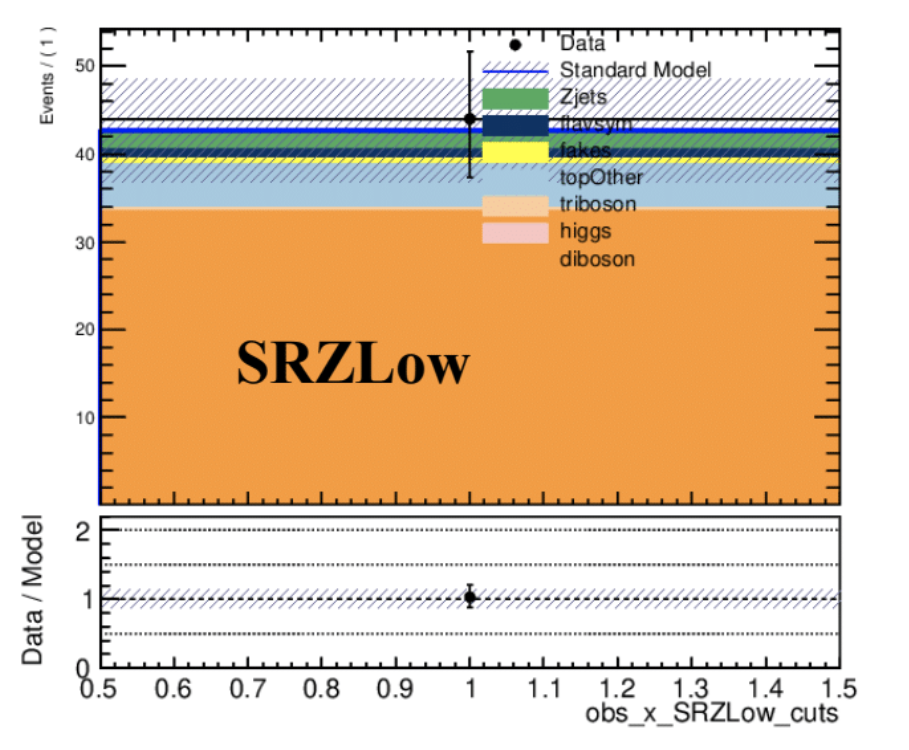
\includegraphics[width=0.45\textwidth]{Images/SUSY/on_Z_low_results.png}
    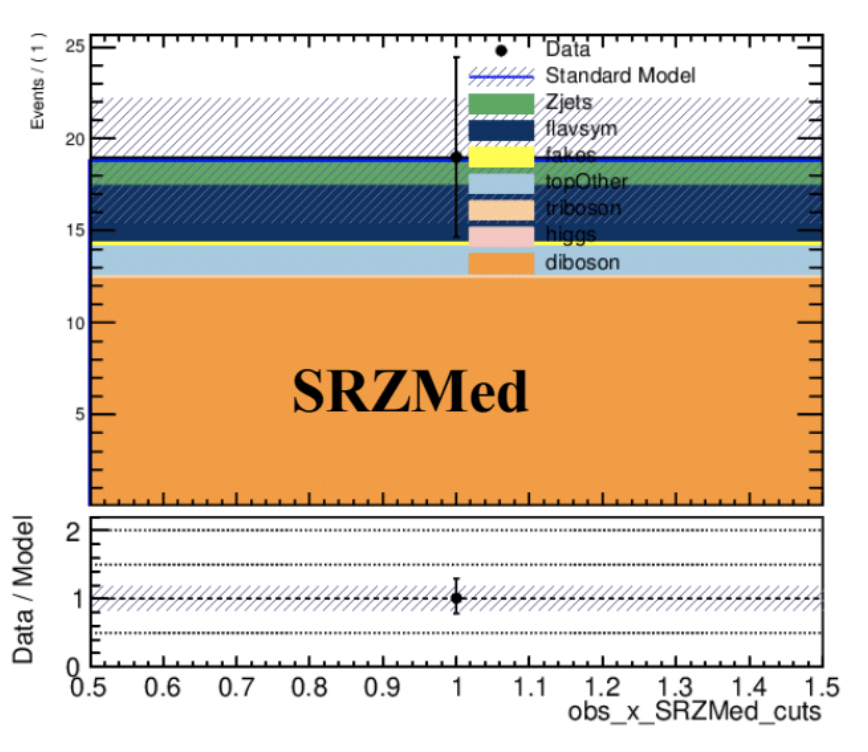
\includegraphics[width=0.45\textwidth]{Images/SUSY/on_Z_med_results.png}
    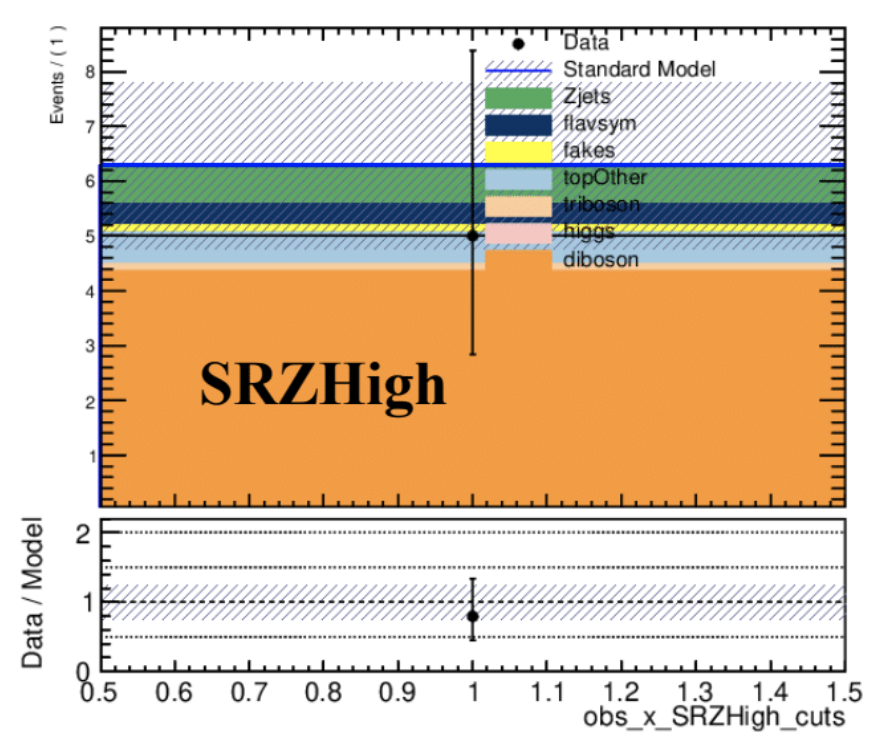
\includegraphics[width=0.45\textwidth]{Images/SUSY/on_Z_high_results.png}
    \caption{Data vs. Standard Model backgrounds for on-Z models. We see that results are within one standard deviation of expected yields.}
    \label{fig:on_Z_results}
\end{figure}

\begin{figure}[htbp]
    \centering
    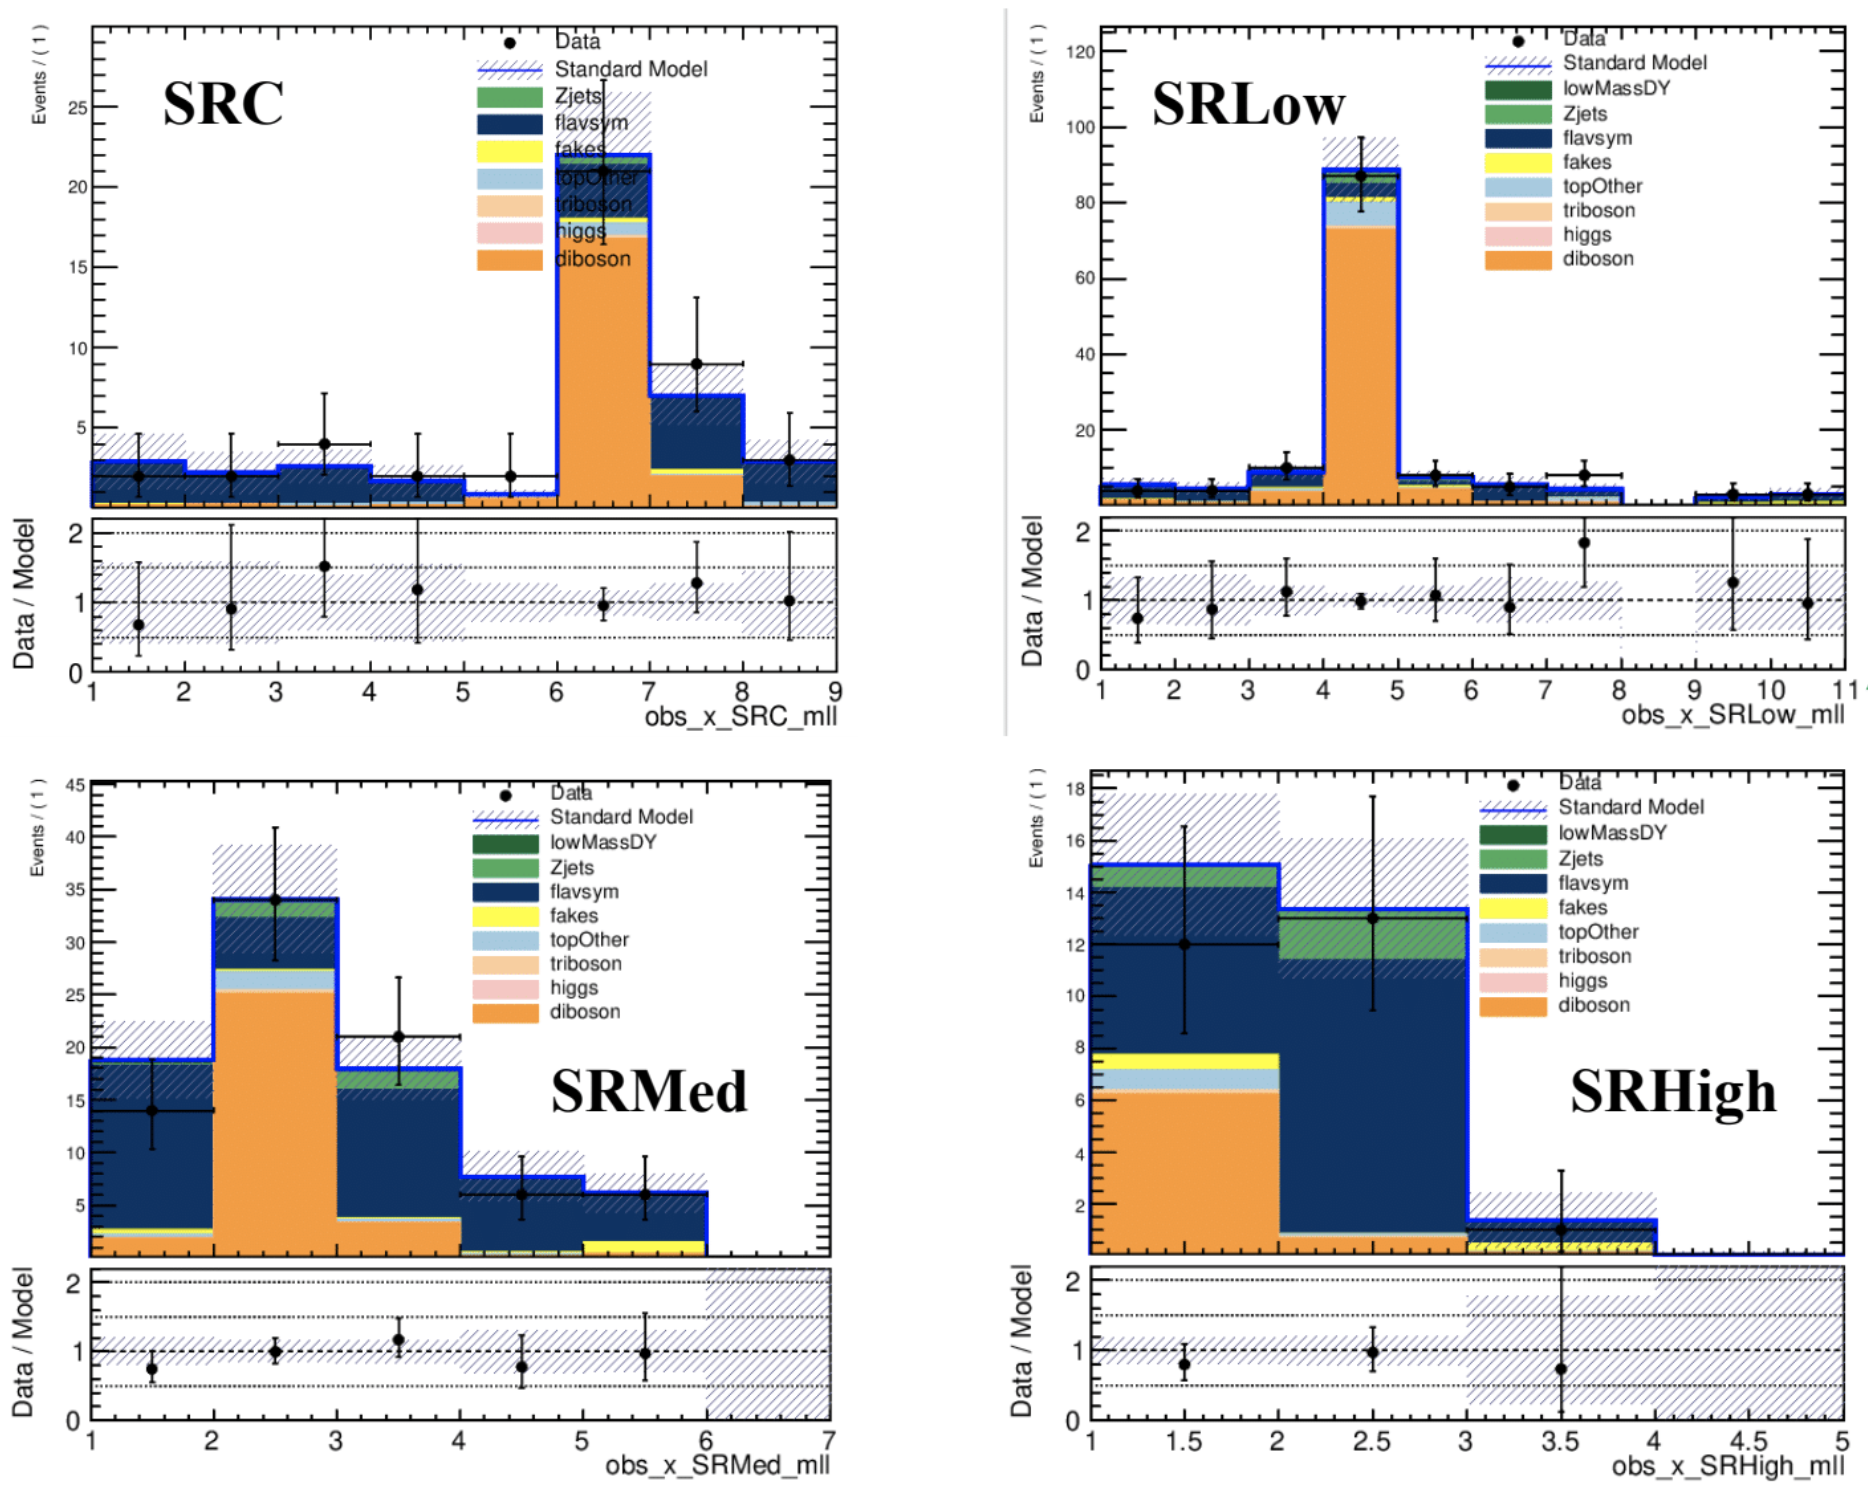
\includegraphics[width=0.85\textwidth]{Images/SUSY/edge_results.png}
    \caption{Data vs. Standard Model backgrounds for edge models. \mll\ is binned on the x axis, using bin sizes which were optimized before unblinding. We see that results are consistent with expected yields and \mll\ shapes.}
    \label{fig:edge_results}
\end{figure}

\begin{figure}[htbp]
    \centering
    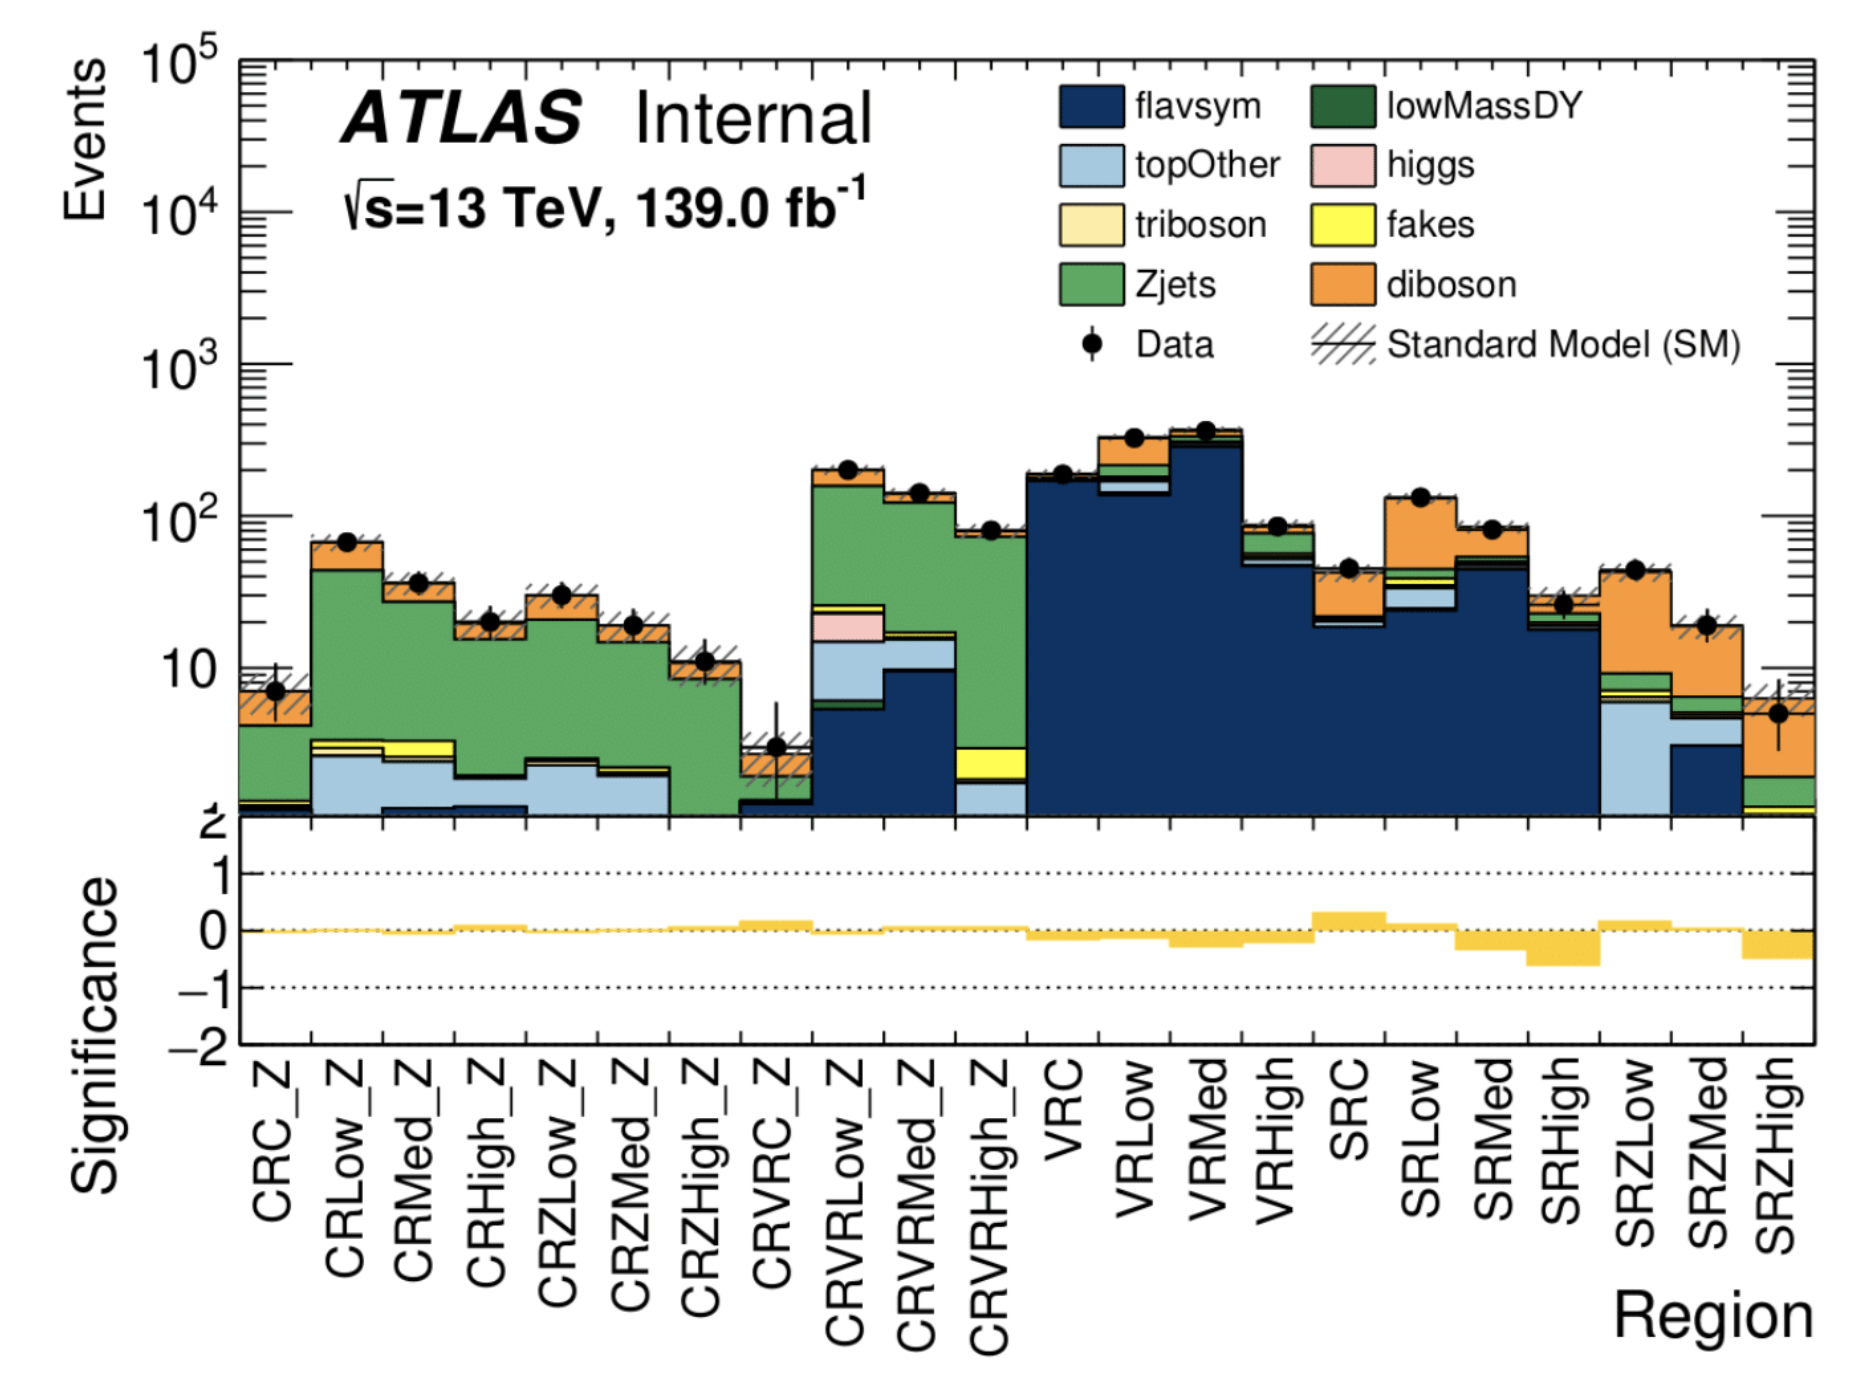
\includegraphics[width=0.85\textwidth]{Images/SUSY/all_results.png}
    \caption{A summary of data vs. Standard Model backgrounds for all regions. We see that data is within one standard deviation of expected yields in all cases.}
    \label{fig:all_results}
\end{figure}